\documentclass[11pt,a4paper]{article}
\usepackage[spanish]{babel}					% Utilizar español
\usepackage[utf8]{inputenc}					% Caracteres UTF-8
\usepackage{graphicx}						% Imagenes
\usepackage[hidelinks]{hyperref}			% Poner enlaces sin marcarlos en rojo
\usepackage{fancyhdr}						% Modificar encabezados y pies de pagina
\usepackage{float}							% Insertar figuras
\usepackage[textwidth=390pt]{geometry}		% Anchura de la pagina
\usepackage[nottoc]{tocbibind}				% Referencias (no incluir num pagina indice en Indice)
\usepackage{amsmath}						% Simbolos matematicos
\usepackage{enumitem}						% Enumeraciones
\usepackage[linesnumbered,ruled,vlined]{algorithm2e}	% Pseudocodigo
\usepackage{listings}

\lstset{
	language=bash
}


% Configuracion de encabezados y pies de pagina
\pagestyle{fancy}
\lhead{Vladislav Nikolov Vasilev}
\rhead{Metaheurísticas}
\lfoot{Grado en Ingeniería Informática}
\cfoot{}
\rfoot{\thepage}
\renewcommand{\headrulewidth}{0.4pt}		% Linea cabeza de pagina
\renewcommand{\footrulewidth}{0.4pt}		% Linea pie de pagina
\decimalpoint								% Hacer que los números decimales usen . en vez de ,

\begin{document}
\pagenumbering{gobble}

% Pagina de titulo
\begin{titlepage}

\begin{minipage}{\textwidth}

\centering

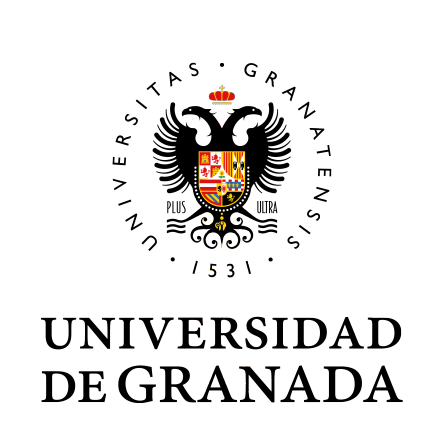
\includegraphics[scale=0.3]{img/ugr.png}\\

\textsc{\Large Metaheurísticas\\[0.2cm]}
\textsc{GRADO EN INGENIERÍA INFORMÁTICA}\\[0.3cm]

\noindent\rule[-1ex]{\textwidth}{1pt}\\[1.5ex]
\textsc{{\Huge PRÁCTICA 1\\[0.1cm]}}
\textsc{{\Large \\Problema del Aprendizaje de Pesos en Características (APC)}}
\noindent\rule[-1ex]{\textwidth}{2pt}\\[3.5ex]

\end{minipage}

\vspace{0.5cm}

\begin{minipage}{\textwidth}

\centering

\textbf{Autor}\\ {Vladislav Nikolov Vasilev}\\[1ex]
\textbf{NIE}\\ {X8743846M}\\[1ex]
\textbf{E-Mail}\\ {vladis890@gmail.com}\\[1ex]
\textbf{Grupo de prácticas}\\ {MH3 Jueves 17:30-19:30}\\[1ex]
\textbf{Rama}\\ {Computación y Sistemas Inteligentes}\\[1ex]
\vspace{0.2cm}


\includegraphics[scale=0.3]{img/etsiit.jpeg}

\vspace{0.3cm}
\textsc{Escuela Técnica Superior de Ingenierías Informática y de Telecomunicación}\\
\vspace{1cm}
\textsc{Curso 2018-2019}
\end{minipage}
\end{titlepage}

\pagenumbering{arabic}
\tableofcontents
\thispagestyle{empty}				% No usar estilo en la pagina de indice

\newpage

\setlength{\parskip}{1em}

\section{Descripción del problema}

El problema que se aborda en esta práctica es el Aprendizaje de Pesos en Características (APC). Es un problema típico de
\textit{machine learning} en el cuál se pretende optimizar el rendimiento de un clasificador basado en vecinos más cercanos.
Esto se consigue mediante la ponderación de las características de entrada con un vector de pesos $W$, el cuál utiliza
codificación real (cada $w_i \in W$ es un número real), con el objetivo de modificar sus valores a la hora de calcular la
distancia. Cada vector $W$ se expresa como $W = \lbrace w_1, w_2, \dots , w_n \rbrace$, siendo $n$ el número de dimensiones
del vector de características, y cumpliéndose además que $\forall w_i \in W, \; w_i \in [0, 1]$.\par

El clasificador considerado para este problema es el 1-NN (genéricamente, un clasificador $k$-NN, con $k$ vecinos, siendo
en este caso $k = 1$), es decir, aquél que clasifica un elemento según su primer vecino más cercano utilizando alguna medida
de distancia (en este caso, utilizando la distancia Euclídea). Cabe destacar que no en todos los casos se usará el clasificador
1-NN ya que se pueden dar casos en los que el vecino más cercano de un elemento sea él mismo. Por ese motivo, en algunas
técnicas/algoritmos se usará un 1-NN con el criterio de \textit{leave-one-out}, es decir, que se busca el vecino más cercano
pero excluyéndose a él mismo.\par

El objetivo propuesto es aprender el vector de pesos $W$
mediante una serie de algoritmos, de tal forma que al optimizar el clasificador se mejore tanto la precisión de éste como su
complejidad, es decir, que se considere un menor número de características. Estos dos parámetros, a los que llamaremos $tasa\_
clas$ y $tasa\_red$, respectivamente, se pueden expresar de la siguiente forma:

\[tasa\_clas = 100 \cdot \frac{nº \; instancias \; bien \; clasificadas \; en \; T}{nº \; instancias \; en \; T}\]
\[tasa\_red = 100 \cdot \frac{nº \; valores \; w_i < 0.2}{nº \; caracteristicas}\]

\noindent siendo $T$ el tamaño del conjunto de datos sobre que el que se evalúa el clasificador.\par

Por tanto, al combinarlos en una única función a la que llamaremos $F(W)$, la cuál será nuestra función objetivo a optimizar
(maximizar), tenemos que:

\[F(W) = \alpha \cdot tasa\_clas(W) + (1 - \alpha) \cdot tasa\_red(W)\] 

\noindent siendo $\alpha$ la importancia que se le asigna a la tasa de clasificación y a la de reducción, cumpliendo que
$\alpha \in [0, 1]$. En este caso, se utiliza un $\alpha = 0.5$ para dar la misma importancia a ambos, con lo cuál se pretende
que se reduzcan al máximo el número de características conservando una $tasa\_clas$ alta.

\section{Descripción de los algoritmos}

Primeramente, antes de empezar con la descripción formal de los algoritmos implementados, vamos a describir algunos aspectos
comunes, como por ejemplo cómo se representan las soluciones, como se inicializan en algunos de los casos y algunas funciones
utilizadas en muchas partes del código, como por ejemplo la función objetivo. Cabe destacar que muchos de los pseudocódigos
que aparezcan a continuación, no se encuentren como tal en la implementación, ya que ya hay funciones que se encargan de
hacerlos.

Como se dijo al principio, cada solución es un vector $W$ en el que $\forall w_i \in W, \; w_i \in [0, 1]$. Por tanto, para
evitar que las soluciones se salgan de este intervalo, se ha implementado una función que se encarga de normalizar los valores
de $W$ en el rango. La función se ha usado, por ejemplo, en la búsqueda local, para hacer que al aplicar el operador
de generación de un nuevo vecino la solución siguiese siendo válida. La implementación de esta función es la siguiente:

\begin{algorithm}[H]
\caption{Función de normalización de $W$}
\SetKwInOut{Input}{input}
\SetKwInOut{Output}{output}
\SetKwProg{NormalizarW}{NormalizarW}{}{}

\NormalizarW{$(W)$}{
\Input{Vector de pesos $W$}
\Output{Vector de pesos $W$ normalizado en $[0, 1]$}

\ForEach{$w_i \in W$}{
	\If{$w_i < 0$}{
		$w_i \gets 0$
	}
	\ElseIf{$w_1 > 1$}{
		$w_i \gets 1$
	}
}

\Return{$W$}
}
\end{algorithm}

Como se ha mencionado anteriormente, también se tienen que generar las soluciones iniciales. En el caso del algoritmo greedy
\textit{RELIEF}, se ha tenido que generar un $W$ inicial en el que todos sus elementos son 0. Conceptualmente, en el siguiente
pseudocódigo se puede ver cuál es la idea que hay detrás:

\begin{algorithm}[H]
\caption{Inicialización de un vector de pesos $W$ en \textit{RELIEF}}
\SetKwInOut{Input}{input}
\SetKwInOut{Output}{output}
\SetKwProg{GenerarWRelief}{GenerarWRelief}{}{}

\GenerarWRelief{$(N)$}{
\Input{Número de características $N$}
\Output{Vector de características $W$ con valores 0}
$W \gets$ vector[$N$]

\ForEach{$w_i \in W$}{
	$w_i \gets 0$
}
\Return{$W$}
}
\end{algorithm}

En el caso de la búsqueda local, para inicializar los valores de $W$ se han generado valores distribuidos uniformemente en
el rango $[0, 1]$. Para mostrar como sería eso conceptualmente, aquí se muestra un pequeño pseudocódigo:

\begin{algorithm}[H]
\caption{Inicialización de un vector de pesos $W$ en BL}
\SetKwInOut{Input}{input}
\SetKwInOut{Output}{output}
\SetKwProg{GenerarWBL}{GenerarWBL}{}{}

\GenerarWBL{$(N)$}{
\Input{Número de características $N$}
\Output{Vector de características $W$ con valores aleatorios}

$W \gets$ vector[$N$]

\ForEach{$w_i \in W$}{
	$w_i \gets$ ValorAleatorioUniformeRango0-1()
}
\Return{$W$}
}

\end{algorithm}

Una vez que sabemos como se representa e inicializa el vector de pesos $W$, vamos a comentar algunos detalles extra. Es
importante saber como se calcula la distancia a un vecino, ya que esto juega un factor muy importante a la hora de encontrar
cuál es el vecino más cercano a un elemento (o el vecino más cercano por el criterio \textit{leave-one-out}). En la
implementación de la práctica se ha utilizado un KDTree, que es una estructura de datos parecida a un árbol binario, solo que
de $K$ dimensiones. Por dentro, esta estructura utiliza la distancia Euclídea (distancia en línea recta entre
dos elementos) para determinar cuál es el elemento más próximo a otro. No hace falta conocer como se implementa esta estructura
de datos, pero sí es importante conocer cómo se realiza el cálculo de la distancia Euclídea. En el siguiente pseudocódigo se
puede ver el cálculo:

\begin{algorithm}[H]
\caption{Cálculo de la distancia Euclídea entre dos puntos}
\SetKwInOut{Input}{input}
\SetKwInOut{Output}{output}
\SetKwProg{DistanciaEuclidea}{DistanciaEuclidea}{}{}

\DistanciaEuclidea{$(e_1, e_2)$}{
\Input{$e_1, e_2$ dos puntos entre los que calcular la distancia}
\Output{Distancia Euclídea}

$distancia \gets \sqrt{\sum_{i=1}^{N} (e_1^i - e_2^i)^2}$

\Return{$distancia$}

}

\end{algorithm}

Y ya sabiendo todo esto, solo nos queda comentar la función objetivo, $F(W)$, que es lo que se pretende optimizar. Para evaluar
la función objetivo, necesitamos calcular $tasa\_clas$ y $tasa\_red$. Para calcular lo primero, podemos seguir la idea
detrás del siguiente pseudocódigo:

\begin{algorithm}[H]
\caption{Cálculo de la tasa de clasificación}
\SetKwInOut{Input}{input}
\SetKwInOut{Output}{output}
\SetKwProg{CalculoTasaClas}{CalculoTasaClas}{}{}

\CalculoTasaClas{$(y, pred, N)$}{
\Input{ $y$ las etiquetas originales, $pred$ las etiquetas predichas y $N$ el número de etiquetas}
\Output{Tasa de elementos bien clasificados}
$bien\_clasificados \gets 0$

\For{$i \gets 1$ \KwTo $N$}{
	\If{$y_i = pred_i$}{
		$bien\_clasificados \gets bien\_clasificados + 1$
	}
}

$tasa\_clas \gets bien\_clasificados \; / \; N$

\Return{$tasa\_clas$}
}

\end{algorithm}

Para calcular $tasa\_red$, suponiendo que queremos saber el número de características por debajo de $0.2$ podemos seguir un
esquema como el siguiente:

\begin{algorithm}[H]
\caption{Cálculo de la tasa de reducción}
\SetKwInOut{Input}{input}
\SetKwInOut{Output}{output}
\SetKwProg{CalculoTasaRed}{CalculoTasaRed}{}{}

\CalculoTasaRed{$(W, N)$}{
\Input{$W$ el vector de pesos $N$ el número de pesos}
\Output{Tasa de reducción}
$carac\_red \gets 0$

\ForEach{$w_i \in W$}{
	\If{$w_i < 0.2$}{
		$carac\_red \gets carac\_red + 1$
	}
}

$tasa\_red \gets carac\_red \; / \; N$

\Return{$tasa\_red$}
}

\end{algorithm}

Y finalmente, para poder calcular la función a optimizar (nuestra función \textit{fitness} u objetivo), teniendo en cuenta que
usamos un $\alpha = 0.5$ para ponderar las dos tasas, y que anteriormente hemos calculado ambas tasas, podemos seguir el
siguiente esquema:

\begin{algorithm}[H]
\caption{Cálculo de la función objetivo o \textit{fitness}}
\SetKwInOut{Input}{input}
\SetKwInOut{Output}{output}
\SetKwProg{CalculoFuncionFitness}{CalculoFuncionFitness}{}{}

\CalculoFuncionFitness{$(tasa\_clas, tasa\_red, \alpha)$}{
\Input{Recibe $tasa\_clas$ y $tasa\_red$ y calcula la agrupación de ambas con un factor $\alpha$}
\Output{Valor \textit{fitness} o agrupación}

$fitness \gets \alpha \cdot tasa\_clas + (1 - \alpha) \cdot tasa\_red$

\Return{$fitness$}

}
\end{algorithm}

Una vez sabiendo todo esto, podemos comenzar a describir las implementaciones de los algoritmos utilizadas.

\subsection{Algoritmos de comparación}

Para la comparación de la metaheurística implementada, utilizaremos dos algoritmos/técnicas:

\begin{itemize}[label=\textbullet]
	\item Un clasificador 1-NN clásico, sin ponderar las características.
	\item Un algoritmo greedy llamado \textit{RELIEF} para el cálculo de los pesos con los que ponderar las características,
	y posteriormente utilizar un 1NN con los valores ponderados.
\end{itemize}

Comencemos por la base: el 1-NN. Este clasificador lo que hace es, dado un conjunto de valores $X$ que pertenecen a 
una muestra y un elemento $e$, decir cuál es el $x \in X$ más cercano a $e$, y por tanto, decir que $e$ pertenece a la
misma clase $x$. Para determinar cuál es el elemento más cercano se puede usar alguna métrica de distancia, como por ejemplo
la distancia Euclídea, descrita anteriormente. A la hora de implementarlo, para poder acelerar los cálculos, se puede usar
un KDTree, ya que permite realizar una consulta rápida (en los casos más favorables su complejidad temporal es $\mathcal{O}
(\log n)$, mientras que en el peor caso es $\mathcal{O}(n)$) utilizando la distancia Euclídea para determinar el vecino más
cercano, con la penalización de que tarda un tiempo $\mathcal{O}(n)$ en ser construido. Para poder ver un esquema de su funcionamiento, se ofrece el siguiente pseudocódigo:

\begin{algorithm}[H]
\caption{Clasificador 1-NN}
\SetKwInOut{Input}{input}
\SetKwInOut{Output}{output}
\SetKwProg{KNN}{1-NN}{}{}

\KNN{$(X, y, e)$}{
\Input{$X$ un conjunto de elementos que pertenecen a una muestra, $y$ las etiquetas correspondientes a cada $x_i \in X$, $e$
el elemento del que buscar su vecino más cercano}
\Output{Clase a la que pertence el vecino más cercano de $e$}

$arbol\_kd \gets$ KDTree($X$)

$x \gets arbol\_kd$.VecinoMasCercano($e$)

$etiqueta \gets y[x]$

\Return{$etiqueta$}

}
\end{algorithm}

Una vez habiendo explicado el 1-NN, vamos a hablar del algoritmo para el cálculo de pesos \textit{RELIEF}. Es un algoritmo
greedy que, comenzando con un $W$ cuyos pesos valen 0, actualiza $W$ para cada $x_i \in X$, buscando para cada $x_i$ cuál es
su aliado más cercano (elemento que tiene la misma etiqueta que $x_i$ con el criterio de \textit{leave-one-out}, ya que él
mismo podría ser su vecino más cercano) y su enemigo más cercano (elemento que tiene diferente etiqueta a la que tiene $x_i$).

A la hora de implementarlo, vamos a utilizar 2 KDTree en cada iteración que se van a construir sobre la marcha. En uno se
encontrarán todos los aliados de $e$ y en el otro estarán todos sus enemigos. Esto puede suponer una gran penalización por el
tiempo de creación de los árvoles, pero es un tiempo insignificante ya que el algoritmo es muy rápido. Después de construir los
árboles, se buscará en el caso del aliado más cercano, por el criterio de \textit{leave-one-out}, cuál es el índice de este
aliado. En el caso del enemigo más cercano, como este no puede ser él mismo, se buscará el índice del vecino más cercano en ese
árbol. Una vez hecho eso, obtendremos los respectivos aliado y enemigo del conjunto de aliados y enemigos. Una vez teniéndolos,
ya se puede actualizar el valor de $W$.

Cuando se ha terminado de iterar sobre todos los elementos de $X$, se normaliza $W$ para que esté en el rango $[0, 1]$ 
eligiendo el $w_i \in W$ que sea más grande. Todos aquellos valores por debajo de 0 se truncan a 0, y el resto se normaliza
dividiéndolos entre $w_m$ (el $w_i$ más grande).

Una vez dicho esto, veamos cómo sería la implementación en pseudocódigo:

\begin{algorithm}[H]
\caption{Cálculo de los pesos mediante \textit{RELIEF}}
\SetKwInOut{Input}{input}
\SetKwInOut{Output}{output}
\SetKwProg{RELIEF}{RELIEF}{}{}

\RELIEF{$(X, Y)$}{
\Input{$X$ un conjunto de elementos que pertenecen a una muestra, $Y$ las etiquetas de cada $x_i \in X$}
\Output{Vector de pesos $W$}
$N \gets $ num. elementos $Y$

$n\_carac \gets $ num. caracteristicas $X$

$W \gets $ GenerarWRelief($n\_carac$)

\For{$i \gets 1$ \KwTo $N$}{
	$x, y \gets X[i], Y[i]$
	
	$aliados \gets e_a \subset X :$ etiqueta($e_a$) $ = y$
	
	$enemigos \gets e_e \subset X:$ etiqueta($e_e$) $ \neq y$
	
	$arbol\_aliados \gets$ KDTree($aliados$)
	
	$arbol\_enemigos \gets$ KDTree($enemigos$)
	
	$aliado\_cercano \gets arbol\_aliados$.ObtenerVecinoMasCercanoL1O($x$)
	
	$enemigo\_cercano \gets arbol\_enemigos$.ObtenerVecinoMasCercano($x$)
	
	$aliado \gets aliados[aliado\_cercano]$
	
	$enemigo \gets enemigos[enemigo\_cercano]$
	
	$W \gets W + \left|x - enemigo\right| - \left|x - aliado\right|$
}

$w_m \gets \max(W)$

\ForEach{$w_i \in W$}{
	\If{$w_i < 0$}{
		$w_i \gets 0$
	}
	\Else{
		$w_i \gets w_i \; / \; w_m$
	}
}
\Return{$W$}
}

\end{algorithm}

\subsection{Algoritmo del método de búsqueda}

A continuación, vamos a estudiar el algoritmo de búsqueda que se ha pedido implementar en esta primera práctica. Se trata de
un algortimo de búsqueda local, que partiendo de un vector $W$ con valores aleatorios busca optimizarlo mediante la
exploración de los vecinos. Esta exploración se realiza modificando con un valor aleatorio generado a partir de una
distribución normal con $\mu = 0$ y $\sigma = 0.3$ un $w_i \in W$, quedándose con el cambio en caso de mejorar la función
objetivo, o descartándolo en otro caso.

Para realizar lo explicado anteriormente, se genera una permutación del conjunto $\lbrace 1, 2, \dots , N \rbrace$, donde $N$
es el número de características, y se van escogiendo las características según el orden de la permutación, aplicándoles
el cambio anteriormente descrito. Si no se produce una mejora, se descarta el cambio realizado. Si no se ha producido mejora
en la función objetivo con la permutación, se escoge una nueva permutación y se repite el proceso, hasta un máximo de $20
\cdot N$ evaluaciones sin éxito seguidas de la función objetivo. Si se produce mejora, se acepta el cambio y se genera una
nueva permutación, repitiendo el proceso. Todo esto se realiza hasta que se hayan realizado 15000 evaluaciones de la función
objetivo, o hasta que se dé la condición anterior (demasiadas iteraciones sin mejora).

La búsqueda local utiliza una función para evaluar lo bueno que es un vector $W$. Esta función lo que hace es aplicar $W$ 
sobre $X$ en aquellas características donde $w_i > 0.2$, y sobre estos crea un KDTree para buscar los índices de los vecinos
más cercanos según el criterio \textit{leave-one-out}. Esta búsqueda, para una mayor velocidad, se aplica sobre todos los
elementos de $X$. Una vez calculados, se obtienen las etiquetas correspondientes, y se realiza la evaluación de la función
objetivo. El pseudocódigo de esta función se puede ver aquí:

\begin{algorithm}[H]
\caption{Función para evaluar $W$ en la búsqueda local}
\SetKwInOut{Input}{input}
\SetKwInOut{Output}{output}
\SetKwProg{Evaluar}{Evaluar}{}{}

\Evaluar{$(X, Y, W$)}{
\Input{$X$ un conjunto de elementos que pertenecen a una muestra, $Y$ las etiquetas de cada $x_i \in X$, $W$ vector de pesos}
\Output{Valor \textit{fitness} para los datos de entrada}
$X\_pesos \gets$ aplicar $w_i \in W$ sobre los $x_i \in X$ donde $w_i > 0.2$

$arbolkd \gets$ KDTree($X\_pesos$)

$vecinos \gets arbolkd$.ObtenerVecinosMasCercanoL1O($X\_pesos$)

$pred \gets Y[vecinos]$

$tasa\_clas \gets$ CalcularTasaClas($Y$, $pred$, num. etiquetas)

$tasa\_red \gets$ CalcularTasaRed($W$, num. caracteristicas)

$fitness \gets$ CalculoFuncionFitness($tasa\_clas$, $tasa\_red$)

\Return{$fitness$}
}

\end{algorithm}

Con todo esto explicado, ya podemos ver el pseudocódigo de la búsqueda local:

\begin{algorithm}[H]
\caption{Cálculo de los pesos mediante la Búsqueda Local}
\SetKwInOut{Input}{input}
\SetKwInOut{Output}{output}
\SetKwProg{BusquedaLocal}{BusquedaLocal}{}{}
\SetKw{Break}{break}
\SetKw{Or}{or}

\BusquedaLocal{$(X, Y)$}{
\Input{$X$ un conjunto de elementos que pertenecen a una muestra, $Y$ las etiquetas de cada $x_i \in X$}
\Output{Vector de pesos $W$}

Inicializar semilla aleatoria

$N \gets $ num. caracteristicas $X$

$W \gets$ GenerarWBL($N$)

$evaluaciones \gets 0$

$evaluacions\_malas \gets 0$

$fitness \gets$ Evaluar($X, Y, W$)

\While{$evaluaciones < 15000$}{
$W\_actual \gets W$

$orden\_caracteristicas \gets $ Permutacion(1 \KwTo $N$)

\ForEach{$carac \in orden\_caracteristicas$}{
	$W[carac] \gets W[carac] +$ GenerarValorDistribucionNormal($\mu$, $\sigma$)
	
	$W \gets$ NormalizarW($W$)
	
	$evaluaciones \gets evaluaciones + 1$
	
	$nuevo\_fitness \gets$ Evaluar($X, Y, W$)
	
	\If{$nuevo\_fitness > fitness$}{
		$fitness \gets nuevo\_fitness$
		
		$evaluaciones\_malas \gets 0$
		
		\Break
	}
	\Else{
		$evaluaciones\_malas \gets evaluaciones\_malas + 1$
		
		$W[carac] \gets W\_actual[carac]$
		
	}
	
	\If{$evaluaciones > 15000$ \Or $evaluaciones\_malas > 20 \cdot N$}{
		\Return{$W$}
	}
}
}

\Return{$W$}
}

\end{algorithm}

\newpage

\section{Desarrollo de la práctica}

La práctica se ha implementado en \textbf{Python3} y ha sido probada en la versión 3.7.1. Por tanto, se recomienda
encarecidamente utilizar un intérprete de Python3 al ejecutar el código y no uno de la versión 2.X, debio a problemas
de compatibilidad con ciertas funciones del lenguaje. Se ha probado el código sobre Linux Mint 19 y al estar basado en
Ubuntu 18 no debería haber problemas de compatibilidad con otros sistemas, además de que Python es un lenguaje muy portable.
No se ha probado en el entorno \textbf{conda}, pero si se consiguen instalar los módulos necesarios, no debería haber
problemas.

A la hora de implementar el software, se han utilizado tanto módulos ya incluidos en Python, como el módulo \textbf{time}
para la medición de tiempos, como módulos científicos y para \textit{machine learning}, como por ejemplo \textbf{numpy} y
\textbf{sklearn}. Este último se ha utlizado para poder dividir los datos para el \textbf{5 Fold Cross Validation}
y para obtener un clasificador KNN que poder utilizar para poder probar los resultados obtenidos por cada uno de los
algoritmos. Para la visualización de datos se ha utilizado \textbf{pandas}, ya que permite conseguir una visualización rápida
de estos gracias a los DataFrames.

Adicionalmente, la estructura de \textbf{KDTree} utilizada ha sido sacada de un módulo externo llamado
\textbf{pykdtree}, cuyo enlace puede ser encontrado en las referencias. Este módulo está implementado en \textbf{Cython} y
\textbf{C} y también utiliza \textbf{OMP}, con lo cuál su rendimiento va a ser muy superior a otras implementaciones como
por ejemplo el \textbf{cKDTree} de \textbf{scipy}\footnote{De hecho, pykdtree está basado en cKDTree y libANN, cogiendo lo
mejor de cada implementación y paralelizando el código con OMP para conseguir unos rendimientos muy superiores a ambos,
tanto a la hora de crear el árbol como para hacer consultas.}. En cuanto a su uso, las funciones y la forma de construirlo
son las mismas que las de cKDTree, con lo cuál se puede consultar su documentación para obtener más información sobre
su uso.

Siendo ahora más concretos en cuanto a la implementación, se ha creado una función para cada uno de los algoritmos que se
han implementado. Estas funciones se encargan de recorrer las particiones creadas y de ejecutar los respectivos
algoritmos pasándoles los datos, además de encargarse de recopilar información estadística para mostrarla luego por
pantalla. Se han utilizado dos semillas aleatorias las cuáles están fijas en el código: una para dividir los datos, y otra en
la búsqueda local, que se fija al principio, justo antes de inicializar los $W$, como se puede ver en el pseudocódigo. Los
ficheros ARFF proporcionados se han convertido al formato CSV con un script propio, con el objetivo de facilitar la lectura
de los datos. Estos archivos también se proporcionan junto con el código fuente implementado.

\newpage

\section{Manual de usuario}

Para poder ejecutar el programa, se necesita un intérprete de \textbf{Python3}, como se ha mencionado anteriormente. Además,
para poder satisfacer las dependencias se necesita el gestor de paquetes \textbf{pip} (preferiblemente \textbf{pip3}).

Se recomienda instalar las dependencias, las cuáles vienen en el archivo \textbf{requirements.txt}, ya que sin ellas, el
programa no podrá funcionar. Se recomienda utilizar el script de bash incluido para realizar la instalación, ya que se
encarga de instalarlo en un entorno virtual para no causar problemas de versiones con paquetes que ya se tengan instaladas en
el equipo o para no instalar paquetes no deseados. Una vez instalados, para poder utilizar el entorno creado se debe ejecutar
el siguiente comando:

\begin{lstlisting}
	$ source ./env/bin/activate
\end{lstlisting}

Para desactivar el entorno virtual, simplemente basta con ejecutar:

\begin{lstlisting}
	(env) $ deactivate
\end{lstlisting}

Para ejecutar el programa basta con ejecutar el siguiente comando:

\begin{lstlisting}
	$ python3 practica1.py [archivo] [algoritmo]
\end{lstlisting}

Los argumentos \textbf{archivo} y \textbf{algoritmo} son obligatorios, y sin ellos el programa lanzará una excepción. En
cuanto a sus posibles valores:

\begin{itemize}[label=\textbullet]
	\item \textbf{archivo} puede ser \textbf{colposcopy}, \textbf{ionosphere} o \textbf{texture}.
	\item \textbf{algoritmo} puede ser \textbf{knn}, \textbf{relief} o \textbf{local}.
\end{itemize}

\begin{figure}[H]
\centering
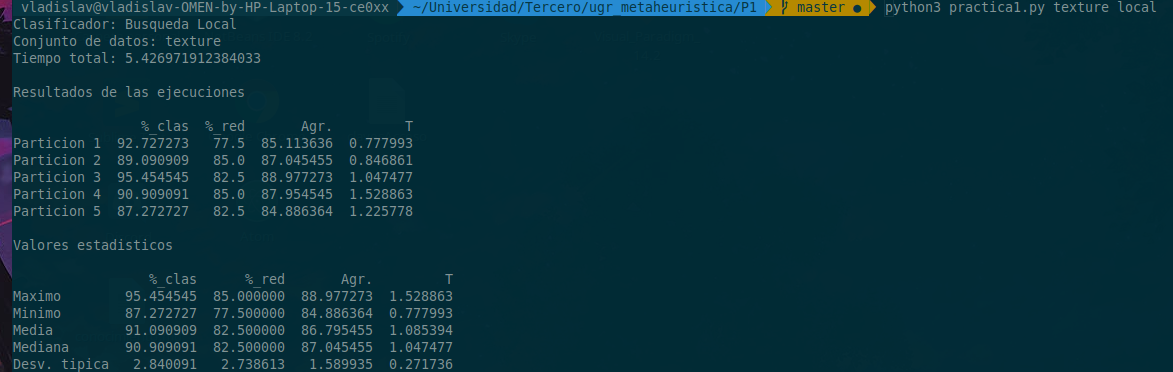
\includegraphics[scale=0.35]{img/out_example.png}
\caption{Ejemplo de salida de la ejecución con los datos \textbf{texture} y el algoritmo \textbf{local}.}
\end{figure}

\newpage

\section{Análisis}

\newpage

\begin{thebibliography}{5}

\bibitem{nombre-referencia}
Texto referencia
\\\url{https://url.referencia.com}

\end{thebibliography}

\end{document}

